\documentclass[a4paper, 11pt]{article}
\usepackage{comment} 
\usepackage{lipsum} %This package just generates Lorem Ipsum filler text. 
\usepackage{fullpage} % changes the margin
\usepackage[a4paper, total={7in, 10in}]{geometry}
\usepackage[fleqn]{amsmath}
\usepackage{amssymb,amsthm}  % assumes amsmath package installed
\newtheorem{theorem}{Theorem}
\newtheorem{corollary}{Corollary}
\usepackage{graphicx}
\usepackage{tikz}
\usetikzlibrary{arrows}
\usepackage{verbatim}
\usepackage[numbered]{mcode}
\usepackage{float}
\usepackage{tikz}
    \usetikzlibrary{shapes,arrows}
    \usetikzlibrary{arrows,calc,positioning}

    \tikzset{
        block/.style = {draw, rectangle,
            minimum height=1cm,
            minimum width=1.5cm},
        input/.style = {coordinate,node distance=1cm},
        output/.style = {coordinate,node distance=4cm},
        arrow/.style={draw, -latex,node distance=2cm},
        pinstyle/.style = {pin edge={latex-, black,node distance=2cm}},
        sum/.style = {draw, circle, node distance=1cm},
    }
\usepackage{xcolor}
\usepackage{mdframed}
\usepackage[shortlabels]{enumitem}
\usepackage{indentfirst}
\usepackage{hyperref}
\usepackage[capitalize, nameinlink]{cleveref}
\renewcommand{\thesubsection}{\thesection.\alph{subsection}}

\newenvironment{problem}[2][Problem]
    { \begin{mdframed}[backgroundcolor=gray!20] \textbf{#1 #2} \\}
    {  \end{mdframed}}

\newenvironment{reduction}
    { \begin{mdframed}[backgroundcolor=blue!20] \\}
    {  \end{mdframed}}
% Define solution environment

\newcommand{\hr}{\noindent\rule{7in}{2.8pt}}
\newenvironment{solution}
    {\textit{Solution:}}
    {\clearpage}
\newcommand{\prob}[1]{\begin{mdframed}[backgroundcolor=gray!20] \textbf{Problem #1}\end{mdframed}}
\renewcommand{\qed}{\quad\qedsymbol}
\newcommand{\bit}{\left\{0, 1\right\}}
\newcommand{\enc}{\mathsf{Enc}}
\newcommand{\dec}{\mathsf{Dec}}
\newcommand{\negl}{\mathsf{negl}}
\newcommand{\prf}{\mathsf{PRFAdv}}
\newcommand{\prg}{\mathsf{PRGAdv}}
\newcommand{\poly}{\mathsf{poly}}
\newcommand{\sign}{\mathsf{Sign}}
\newcommand{\verify}{\mathsf{Verify}}
\newcommand{\macvq}{\mathsf{MAC^{vq}}}
\newcommand{\mac}{\mathsf{MAC}}
\newcommand{\func}{\mathsf{Func}}
\newcommand{\AES}{\mathsf{AES}}
\newcommand{\N}{\mathbb{N}}
\newcommand{\R}{\mathbb{R}}
\newcommand{\Z}{\mathbb{Z}}

\newcommand{\calA}{\mathcal{A}}
\newcommand{\calB}{\mathcal{B}}
\newcommand{\calC}{\mathcal{C}}
\newcommand{\calE}{\mathcal{E}}
\newcommand{\calF}{\mathcal{F}}
\newcommand{\calG}{\mathcal{G}}
\newcommand{\calH}{\mathcal{H}}
\newcommand{\calI}{\mathcal{I}}
\newcommand{\calK}{\mathcal{K}}
\newcommand{\calM}{\mathcal{M}}
\newcommand{\calS}{\mathcal{S}}
\newcommand{\calT}{\mathcal{T}}
\newcommand{\calX}{\mathcal{X}}
\newcommand{\calY}{\mathcal{Y}}

\newcommand{\inparen}[1]{\left{ #1 \right}}
\newcommand{\probtwo}[2]{\mathsf{Pr}_{#1}\left[ #2 \right]}
\newcommand{\set}[1]{\left\{ #1 \right\}}
\newcommand{\ct}{\mathsf{ct}}
\newcommand{\twotimessadv}[1]{\mathsf{2SSAdv}\left[ #1 \right]}



\newlength{\protowidth}
\newcommand{\pprotocol}[5]{
{\begin{figure*}[#3]
\begin{center}
\setlength{\protowidth}{\textwidth}
\addtolength{\protowidth}{-3\intextsep}

\fbox{
        \small
        \hbox{\quad
        \begin{minipage}{\protowidth}
    \begin{center}
    {\bf #1}
    \end{center}
        #5
        \end{minipage}
        \quad}

        }
        
\end{center}
\vspace{-4ex}
\caption{{#4} #2}
\end{figure*}
} }

% the first arg is name of security game
% the second arg is caption
% the third arg is the game description
% the label needs to be included 
\newcommand{\securitygame}[4]{
   \pprotocol{#1}{#2}{ht!}{#3}{#4}
}

\newcommand{\constr}[4]{
   \pprotocol{#1}{#2}{tbh!}{#3}{#4}
}

\begin{document}

\noindent
\large\textbf{Anish Banerjee, Shankh Gupta} \hfill \textbf{Problem Set - 2}   \\
\normalsize COL759: Cryptography \hfill September 2023\\
\hr


\prob{1: Cryptosystems secure against side-channel attacks}
\begin{solution}
    Consider the PRF $F':\bit^{n+1}\times\bit^n\rightarrow\bit^n$
    $$F'(k||b_k,x)=
        \begin{cases}
            F(k,0^n)[1\dots n-1]||b_k \hspace{50pt} \text{if } x=0^n \\
            F(k,x) \hspace{120pt} \text{Otherwise}
        \end{cases}$$
    In other words, the last bit of $F(k,0^n)$ has been replaced with the last bit of the key.

    \begin{enumerate}[(a)]
        \item Let $\calA$ be an adversary which breaks the PRF security of $F'$ with non-negligible advantage $\epsilon$. We will build a reduction $\calB$ which breaks the PRF security of $F$ with the same advantage.
              \securitygame{Problem 1(a)}{Reduction for Problem 1(a)}{\label{red:p1a}}
              {
                  \begin{itemize}
                      \item Challenger picks a uniformly random bit $b \gets \bit$ and a key $k\gets \calK$.
                      \item $\calB$ samples a random $b_k \gets \bit$.
                      \item The adversary $\calA$ makes polynomially many queries $\{x_i\}$ to $\calB$ who passes them to the challenger. Challenger replies as in the PRF Game.
                      \item Upon receiving the response $y_i$ of each query, $\calB$ checks if $x_i=0$. If so, it modifies $y_i$ by exchanging its last bit with $b_k$. Otherwise, it just passes $y_i$ to $\calA$.
                      \item After polynomially many queries, $\calB$ forwards the response send by $\calA$ $(b')$ and wins if $b=b'$.
                  \end{itemize}
              }
              \begin{figure}[!ht]
                  \centering
                  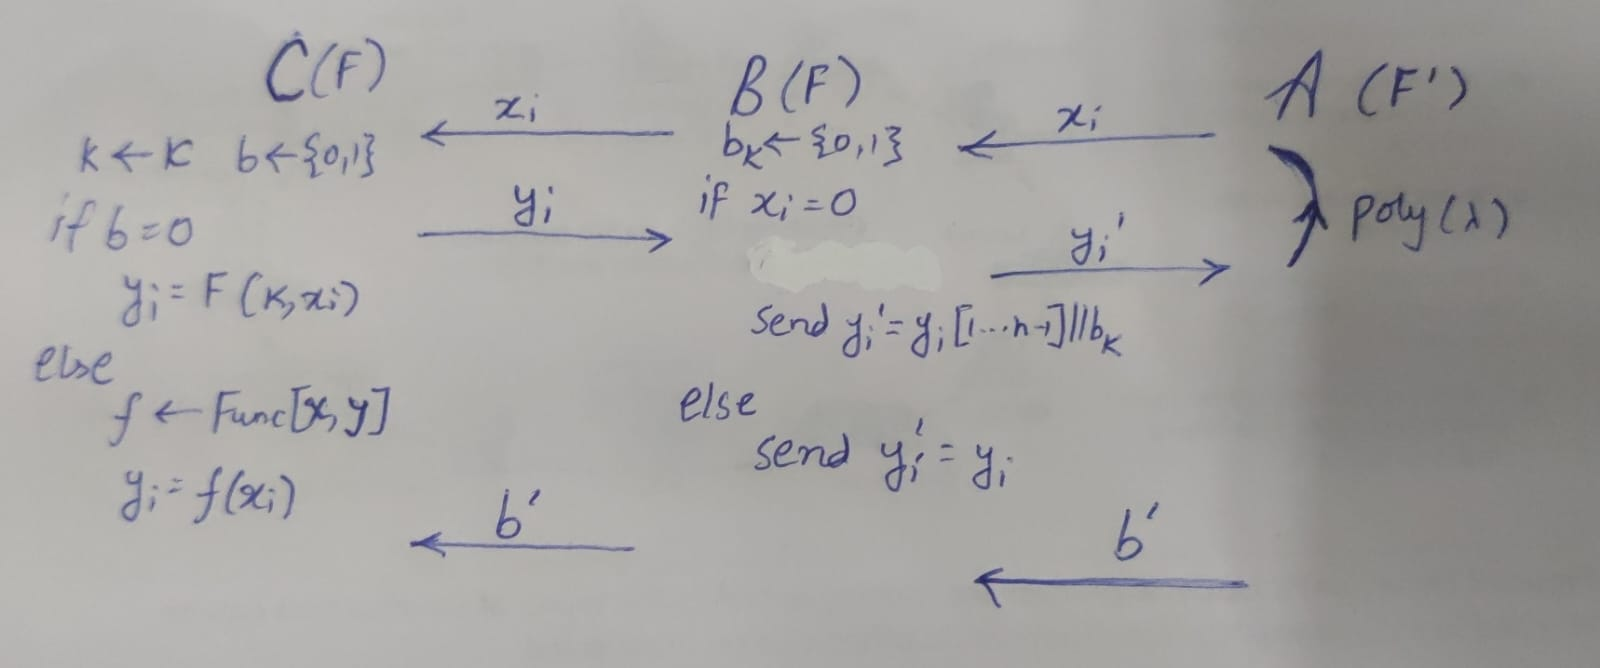
\includegraphics[scale=0.25]{images/Reduction1.jpg}
                  \caption{Image for Problem 1(a)}
                  \label{fig:red1}
              \end{figure}

              When the challenger chooses $b=0$, the game is equivalent to the challenger choosing 0 in PRF game of $F'$.
              \begin{center}
                  Pr[$b'=0|b=0$]=Pr[$\calA$ outputs zero when the challenger chooses 0 in PRF game of $F'$]
              \end{center}
              When the challenger chooses $b=1$, $\calA$ receives the output of a random function for all $x_i\neq0^n$. For $x_i=0^n$, the output received is $r||b_k$. Since $b_k$ is choosen randomly, this too is random.
              \begin{center}
                  Pr[$b'=0|b=1$]=Pr[$\calA$ outputs zero when the challenger chooses 1 in PRF game of $F'$]
              \end{center}
              Hence we can conclude,
              $$\prf[\calB,F]=\prf[\calA,F']$$

        \item We will show that $F'$ does not satisfy 1-leakage resilience by constructing an adversary $\calA'$ who makes a leakage query for the last bit of the key and breaks $F'$.
              \begin{itemize}
                  \item \textbf{Leakage Query:} $\calA'$ makes a query for the last bit of the key and receives $b_k$ from the challenger.
                  \item \textbf{PRF Query:} $\calA'$ queries for the $x=0^n$ and receives $y_i$. He checks if the last bit of $y_i$ is $b_k$. If yes it outputs $b'=0$ (PRF), otherwise it outputs $b'=1$ (Random Function).
              \end{itemize}
              From the game and definition of $F'$, it is evident that:
              $$\Pr[b'=0|b=0]=1$$
              When the challenger chooses $b=0$, the evaluation of a random function at $0^n$ can have its last bit as 0 or 1 with 1/2 probability. So,
              $$\Pr[b'=0|b=1]=\frac12$$
              And the advantage of $\calA'$ is
              $$\prf[\calA,F']=\Pr[b'=0|b=0]-\Pr[b'=0|b=1]=1-\frac12=\frac12$$
              Which is non-negligible.
    \end{enumerate}
\end{solution}


\prob{2 : MACs: unique queries vs non-unique queries}
\begin{solution}
    \begin{enumerate}[(a)]
        \item We propose the following MAC scheme $\calI_\text{uq} = (\sign_\text{uq}, \verify_\text{uq})$ that is $\mathsf{UFCMA-Unique}$ secure, but not $\mathsf{UFCMA}$ secure :
              $$\sign(k, m; r) = (r, F(k_1, r) || F(k_2, m \oplus r))$$ and
              $$\verify(k, m, (\sigma_0, \sigma_1)) = 
              \begin{cases}
                      1 & \text{if } \sigma_1 = F(k_1, \sigma_0) || F(k_2, m \oplus \sigma_0) \\
                      0 & \text{Otherwise}
                  \end{cases}$$
              where $k = (k_1, k_2) \in \bit^{2n}$, $m \in \bit^n$ and $r \in \bit^n$

        \item To prove the $\mathsf{UFCMA-Unique}$ security of $\calI_\text{uq}$, we first build the following sequence of hybrid games:

              \textit{Game 0:} This is the original security game.
              \begin{itemize}
                  \item \textbf{Setup Phase :} Challenger chooses a PRF key $k = (k_1, k_2)$.
                  \item \textbf{Query Phase :} Adversary sends polynomially many queries. For the $i^{th}$ query $m_i$, the challenger chooses a random string $r_i \leftarrow \bit^n$ and sends $\sigma_i = \sign(k, m_i ; r_i)$ to the adversary.
                  \item \textbf{Forgery :} Finally, the adversary outputs $(m^*, \sigma^*)$ such that $(m^*, \sigma^*) \neq (m_i, \sigma_i)$ for all i.
              \end{itemize}
              Let the winning probability of Adversary $\calA$ in Game 0 be $p_0$.
              \vspace{20pt}

              \textit{Game 1:} In this game, Challenger replaces one of the PRFs with a random function.
              \begin{itemize}
                  \item \textbf{Setup Phase :} Challenger chooses a PRF key $k = (k_1, k_2)$ and samples $f \leftarrow \func[\calX, \calY]$. (here $\calY = \bit^n$ and $\calX = \bit^n$)
                  \item \textbf{Query Phase :} Adversary sends polynomially many queries. For the $i^{th}$ query $m_i$, the challenger chooses a random string $r_i \leftarrow \bit^n$ and sends $\sigma_i = (r_i,f(r_i) || F(k_2, m \oplus r_i))$ to the adversary.
                  \item \textbf{Forgery :} Finally, the adversary outputs $(m^*, \sigma^*)$ such that $(m^*, \sigma^*) \neq (m_i, \sigma_i)$ for all i.
              \end{itemize}
              Let the winning probability of Adversary $\calA$ in Game 1 be $p_1$.
              \vspace{20pt}

              \textit{Game 2:} In this game, Challenger replaces both the PRFs with random functions.
              \begin{itemize}
                  \item \textbf{Setup Phase :} Challenger samples $f_1 \leftarrow \func[\calX, \calY]$ and $f_2 \leftarrow \func[\calX, \calY]$.
                  \item \textbf{Query Phase :} Adversary sends polynomially many queries. For the $i^{th}$ query $m_i$, the challenger chooses a random string $r_i \leftarrow \bit^n$ and sends $\sigma_i = (r_i,f(r_i) || f(m \oplus r_i))$ to the adversary.
                  \item \textbf{Forgery :} Finally, the adversary outputs $(m^*, \sigma^*)$ such that $(m^*, \sigma^*) \neq (m_i, \sigma_i)$ for all i.
              \end{itemize}
              Let the winning probability of Adversary $\calA$ in Game 2 be $p_2$. 
              \vspace{20pt}

              \textbf{Claim 1 :} $|p_0 - p_1|$ is negligible.
              
              \begin{figure}[!ht]
                \centering
                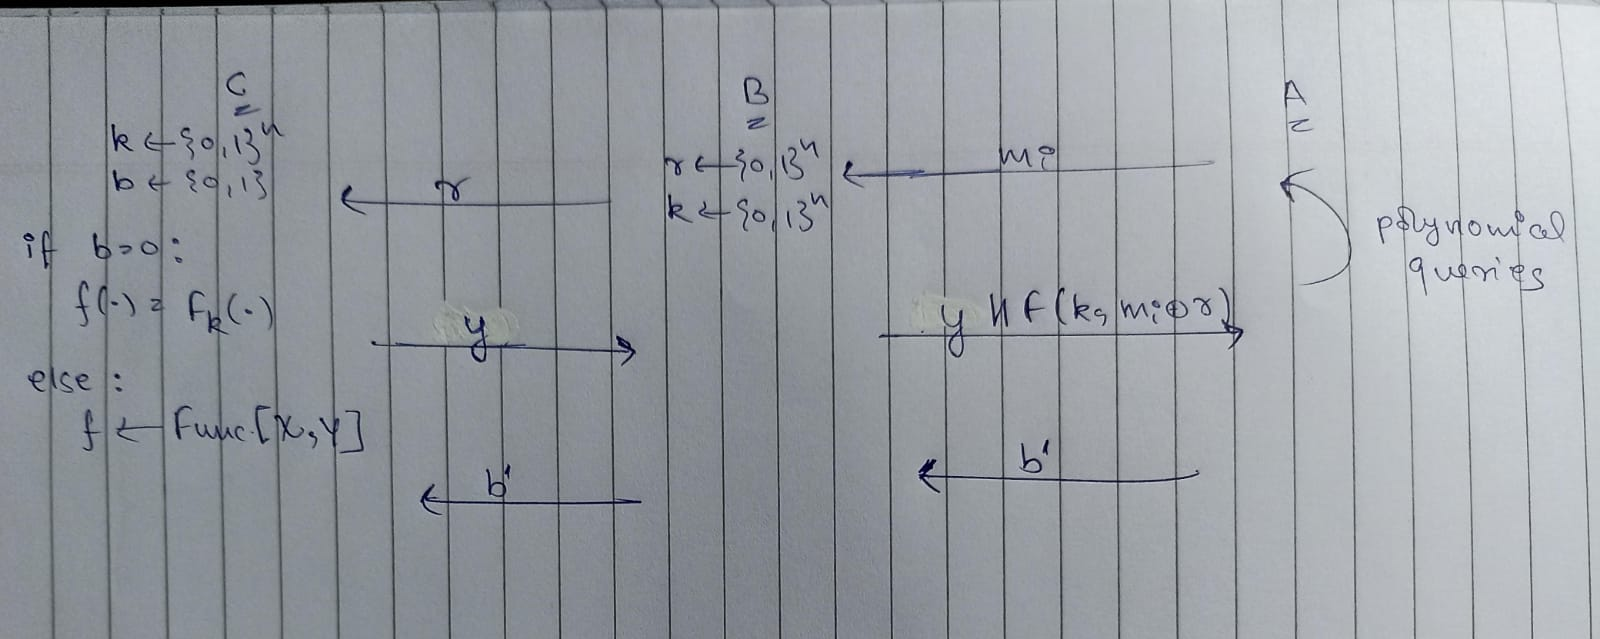
\includegraphics[scale=0.25]{images/Claim1.jpg}
                \caption{Reduction for Claim 1}
                \label{fig:claim1}
              \end{figure}

              \textit{Proof:} Let $\calA$ be an adversary for which the claim is false. We will show a reduction algorithm $\calB$ which uses $\calA$ and has $|p_0 - p_1|$ advantage in the PRF game.

              \begin{itemize}
                \item The reduction algorithm receives signing queries $\{m_i\}$ from $\calA$. 
                \item It samples $r_i$ and a key $k$ and forwards it to the PRF challenger.
                \item It then receives $y_i$ from the PRF challenger and calculates $\sigma_i = (r_i, y_i || F(k, m \oplus r_i))$. It sends the signature $\sigma_i$ to the adversary.
                \item  The adversary then guesses a bit b, where b = 0 for Game 0 and b = 1 for Game 1. The reduction $\calB$ then forwards the bit b to the PRF challenger.
              \end{itemize}
                 

              If the PRF challenger chooses PRF, this corresponds to Game 0 for the adversary $\calA$ and it outputs 0 with a probability $p_0$. On the other hand, if PRF challenger chooses a random function, then it corresponds to Game 1 for the adversary and it outputs 1 with probability $p_1$. 
              So $$\prf[\calB, F] = |p_0 - p_1|$$
              Hence, $|p_0 - p_1|$ is negligible as it is given that $F$ is a secure PRF.

              \textbf{Claim 2:} $|p_1 - p_2|$ is negligible.

              \begin{figure}[!ht]
                \centering
                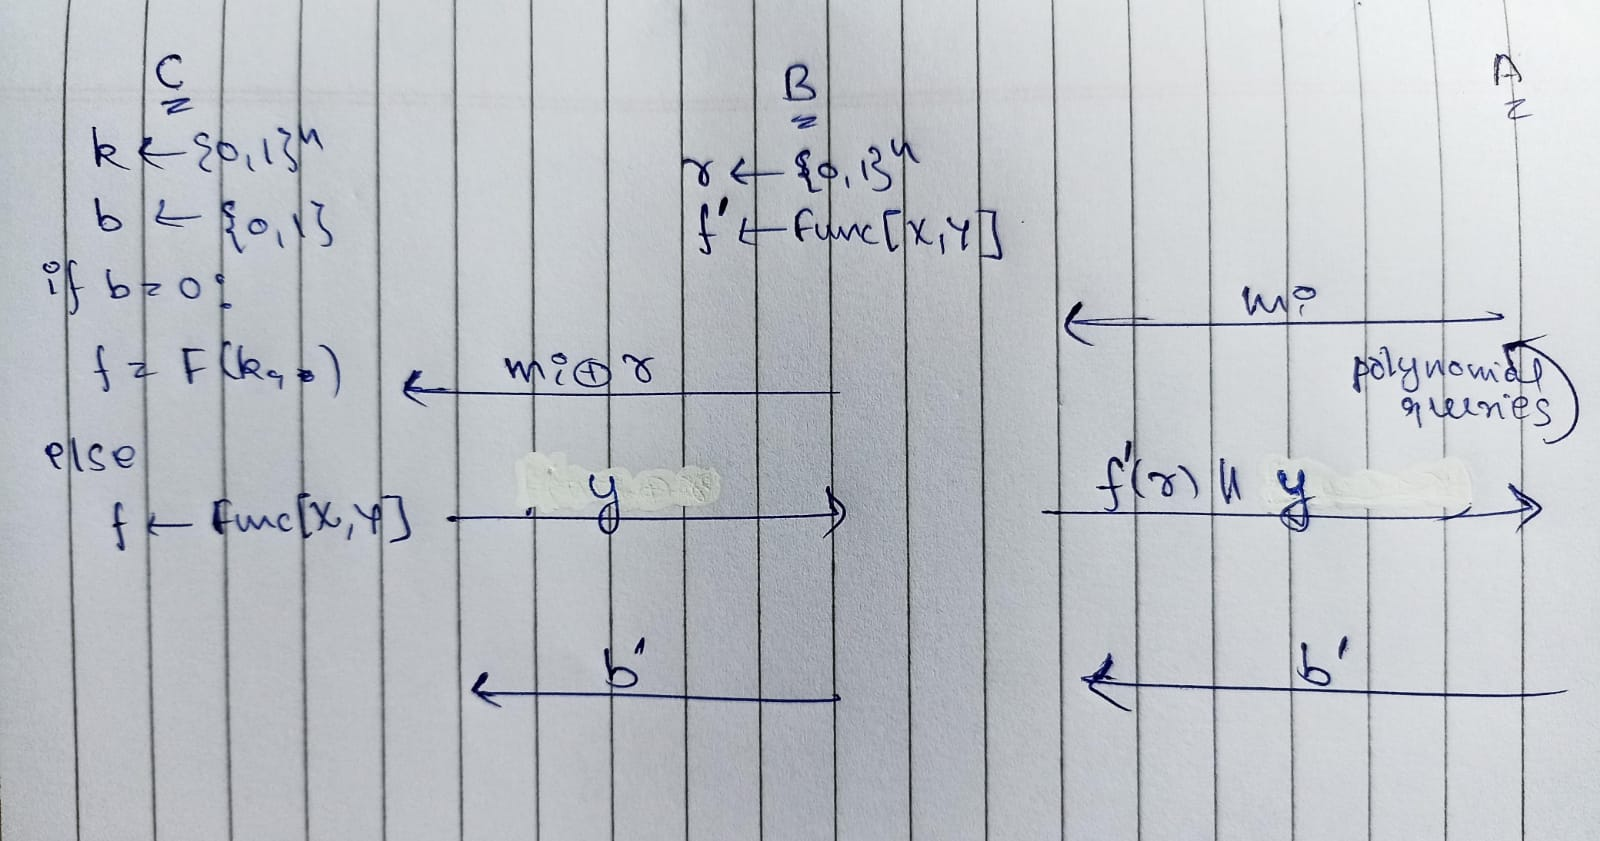
\includegraphics[scale=0.25]{images/Claim2.jpg}
                \caption{Reduction for Claim 2}
                \label{fig:claim2}
              \end{figure}

              \textit{Proof:} Let $\calA$ be an adversary for which the claim is false. We will show a reduction algorithm $\calB$ which uses $\calA$ and has $|p_1 - p_2|$ advantage in the PRF game..
              \begin{itemize}
                \item The reduction algorithm receives signing queries $\{m_i\}$ from $\calA$.
                \item It samples $r_i$ and a random function $f' \leftarrow \func[\calX, \calY]$. It then forwards $m_i \oplus r_i$ to the PRF challenger.
                \item It then receives $y_i$ from the PRF challenger and calculates $\sigma_i = (r_i, f'(r_i) ||y_i)$. It sends the signature $\sigma_i$ to the adversary.
                \item The adversary then guesses a bit b, where b = 0 for Game 1 and b = 1 for Game 2. The reduction $\calB$ then forwards the bit b to the PRF challenger.
              \end{itemize}

              If the PRF challenger chooses PRF, this corresponds to Game 1 for the adversary $\calA$ and it outputs 0 with a probability $p_1$. On the other hand, if PRF challenger chooses a random function, then it corresponds to Game 2 for the adversary and it outputs 1 with probability $p_2$. 
              So $$\prf[\calB, F] = |p_1 - p_2|$$
              Hence, $|p_1 - p_2|$ is negligible as it is given that F is a secure PRF.

              \textbf{Claim 3:} For any Adversary $\calA$, $p_2 = \frac{1}{|\calY|^2}$. (note that, $|\calY| = 2^n$).

              \textit{Proof :} As, $f_1$ and $f_2$ are completely random functions, $f(x)$ for any x is equivalent to choosing a random output $y \in \calY$.

              In order to win the game, the output by the adversary $(m^*, \sigma^*)$ must satisfy $\sigma^*_1 = f_1(r)$ and $\sigma^*_2 = f_2(m_i \oplus r)$ ($\sigma^*_1$ and $\sigma^*_2$ are the first n and the last n bits of $\sigma^*$ respectively). Since $f_1$ and $f_2$ are completely random (and $(m^*,\sigma^*)$ can't be the same as any message-signature pair queried before), the probability of this happening would be $\frac{1}{|\calY|^2}$.

              Thus, by all the above claims, we can prove that $\calI_\text{uq}$ is a $\mathsf{UFCMA-Unique}$ $\mac$ scheme.

        \item We will show this using the following adversary:

              \begin{itemize}
                  \item The adversary queries for $m$ twice and receives 
                  $$\sigma_1 = (r,F(k_1, r) || F(k_2, m \oplus r))$$ 
                  $$\sigma_2 = (r', F(k_1, r') || F(k_2, m \oplus r'))$$
                  \item It then sends $(m \oplus r \oplus r', (r', F(k_1, r') || F(k_2, m \oplus r)))$ as the forgery.
              \end{itemize}

              Since $(m \oplus r \oplus r') \oplus r' = (m \oplus r)$, the above forgery is valid. 
              
              The only case where this forgery would not work is when both $r$ and $r'$ are same. This happens with a very small probability of $\frac{1}{2^{n}}$ and hence is negligible. So the adversary wins with a \textbf{probability of almost 1}.
              So, $\calI_\text{uq}$ is not $\mathsf{UFCMA}$ secure scheme.
              
    \end{enumerate}
\end{solution}


\prob{3 : A mistake in the lecture notes}
\begin{solution}
    According to the given flawed argument, for any (even unbounded) adversary $\calA$ who wins the MAC game with verification queries ($\macvq$) with advantage $\epsilon$, we can construct an adversary $\calB$ who wins the MAC game without verification queries ($\mac$) with probability $\epsilon$. However, we will show an adversary $\calA'$ who wins  $macvq$ with advantage 1 but the reduction $\calB$ cannot use it to win $\mac$.

    The key observation here is that since every message has a unique signature, $\calB$ cannot send a forgery of a message which it has already queried.
    \begin{itemize}
        \item $\calA'$ sends verification queries $(\verify , m, \sigma) \forall \sigma\in\calT$ where $\calT$ is the signature space.
        \item For the first verification query, $\calB$ queries the challenger to obtain the signature $\sigma^\star$, and checks all the verification queries against this.
    \end{itemize}
    One of the queries by $\calA'$ must be $(\verify , m, \sigma^\star)$ and thus he wins the $\macvq$ game. However, $\calB$ cannot use this forgery to win the $\mac$ game since he has already queried it from the challenger.

\end{solution}


\prob{4 : Even-Mansour instantiated with a bad permutation}
\begin{solution}
    The key observation here is that for any query $x_i$ which results in an output $y_i$:
    $$(y_i-k_2)(x_i+k_1)=1 \mod p$$
    So, we query the oracle at 3 points 0,1,2 and form three equations:
    $$(y_0-k_2)(0+k_1)=1 \mod p$$
    $$(y_1-k_2)(1+k_1)=1 \mod p$$
    $$(y_2-k_2)(2+k_1)=1 \mod p$$
    On solving,
    $$k_1=2(y_1-y_2)(y_0+y_2-2y_1)^{-1}$$
    $$k_2=y_1-k_1(y_0-y_1)$$
    Now, we can just query $\pi$ and check if these $(k_1,k_2)$ satisfy $y_i=\pi(x_i+k_1)+k_2$ to distinguish it from a random permutation.

    \noindent\textbf{Note:} all the additions and multiplications are modulo p
\end{solution}


\prob{5 : 3-round Luby-Rackoff with inversion queries}
\begin{solution}
    To launch an attack against the 3-round Luby-Rackoff permutation, we will need 3 oracle queries.
    \begin{itemize}
        \item permute(x, y)
        \item permute(x, z)
        \item inverse\_permute($\alpha$, $\beta$)
    \end{itemize}
    where x, y and z are some 16 bytes array and $y \neq z$. Let permute(x, y) = $(\gamma_1, \delta_1)$ and permute(x, z) = $(\gamma_2, \delta_2)$.

    We will choose $\alpha = \gamma_2$ and $\beta = \delta_2 \oplus y \oplus z$. Let inverse\_permute($\alpha$, $\beta$) = ($m$, $n$).

    If $ m = x \oplus \gamma_1 \oplus \gamma_2$ then the adversary outputs 0 (indicating PRP) else the adversary attack outputs 1 (indicating Completely random).

    This attack works because for 3-round Luby-Rackoff $$PRP(x, y) = (x \oplus F(k_2, y \oplus F(k_1, x)), y \oplus F(k_1, x) \oplus F(k_3, x \oplus F(k_2, y \oplus F(k_1, x))$$
    and
    $$PRP^{-1}(u, v) = (u \oplus F(k_2, v \oplus F(k_3, u), ... )$$

    on substituting $(u, v) = (\alpha, \beta)$ we get $m = x \oplus F(k_2, y \oplus F(k_1, x)) \oplus F(k_2, z \oplus F(k_1, x))$ which is same as $x \oplus \gamma_1 \oplus \gamma_2$.
\end{solution}


\prob{6 : CBC mode with bad initialization}
\begin{solution}
    Suppose the given ciphertext is $(ct_0, ct_1, ct_2)$. Then
    $$ct_0=\AES(k,k\oplus m_0)$$
    $$ct_1=\AES(k,ct_0\oplus m_1)$$
    $$ct_2=\AES(k,ct_1\oplus m_2)$$

    The attacker passes $(ct_0, ct_0, ct_0)$ to the decrypt query and recieves $(m'_0,m'_1,m'_2)$. Note that $m'_0=m_0$ He can simply recover the key by
    $$m'_1=\AES^{-1}(ct_0)\oplus ct_0=k\oplus m'_0\oplus ct_0$$
    $$\implies k=m'_1\oplus m'_0\oplus ct_0$$
\end{solution}


\prob{Part B : Coding Problem-Padding Oracle Attack}
The concept here is similar to the padding oracle attack discussed in class. First, we find the padding of the message corresponding to the given ciphertext. For this, we begin from the end of the first 16 byte block of the ciphertext (after the initialization vector) and manipulate each byte till we get a padding error. For instance, in the example given in the problem statement:
$$m' = (10, 10, 10, 10, 10, 10, 10, 10, 10, \mathbf{10}, 11, 42, 33, 01, 89, 12)$$
If the highlighted byte is altered, then it will result in a padding error. But if the bytes after the highlighted one are altered, there will be no padding error.

Let the number of padding bytes be $p$. Now, to decipher the $(p+1)^\text{th}$ byte, we increase the padding bits by 1. This will result in a padding error. So, we check for which $k$
$$m'_{p+1}\oplus k = p+1$$
When this happens, the padding error will stop since the first $p+1$ bytes have the value $p+1$. The message byte can be recovered simply as
$$m'_{p+1} = (p+1)\oplus k$$
This process is continued till we get the entire message.
\end{document}
